%
% zahlensysteme.tex
%
% (c) 2020 Prof Dr Andreas Müller, Hochschule Rapperswil
%
\section{Zahlensysteme
\label{buch:section:zahlensysteme}}
\rhead{Zahlensysteme}
Auf modernen Allzweck-Prozessoren steht eine ganze Reihe verschiedener
numerischer Datentypen mit unterschiedlichen Eigenschaften
bezüglich Geschwindigkeit und Fehlerverhalten zur Verfügung.
In diesem Abschnitt sollen sie vorgestellt und miteinander verglichen
werden.
Es gilt, den für eine Berechnung zweckmässigsten Typen zu wählen,
wobei Speicherbedarf, Laufzeit und Parallelisierbarkeit wesentliche
Aspekte sind.

Microcontroller sind im Vergleich zu Allzweckprozessoren oft stark
\index{Microcontroller}%
eingeschränkt.
Meist sind nur Ganzahltypen mit oft sehr beschränkter Länge implementiert.
Manchmal kann die Arithmetik-Einheit des Prozessors nicht einmal eine
Multiplikation in Hardware ausführen, sie muss in Software nachgebildet
werden.
Für Floatingpoint Operationen muss oft Bibliotheken zurückgegriffen
werden, die den Speicherbedarf erhöhen und langsam sind.
Die Implementation von numerischen Berechnungen in eingebetteten Anwendungen
ist daher mit besonderen Herausforderungen konfrontiert.

Dieselbe Schwierigkeit haben auch Allzweck-Prozessoren wenn die
Genauigkeitsanforderungen die Möglichkeiten der von der Prozessor-Hardware
implementierten Typen übersteigt.
Dieser Fall tritt beispielsweise bei Berechnungen in der Kryptographie auf,
wo oft mit Ganzzahlen mit Tausenden von Stellen gerechnet werden muss.
Im Abschnitt~\ref{buch:subsection:mp} mit der GNU Multiprecision-Library
ein Beispiel einer Bibliothek vorgestlelt.

\subsection{Zahlendarstellung bezüglich verschiedener Basen
\label{buch:subsection:basen}}
Allen Zahlensystemen gemeinsam ist die Positionsdarstellung.
\index{Positionsdarstellung}
Eine Zahl wird als Zeichenkette $x=x_nx_{n-1}\dots x_3x_2x_1x_0$ mit
wobei die Zeichen $x_i$ Ziffern mit $0 \le x_i < b$ sind.
$b$ ist die Basis des Zahlensystems.
Der Wert der Zahl $x$ ist dann 
\[
x
=
\sum_{k=1}^n x_kb^k.
\]
Wir hängen die Basis also Index an eine Zahlendarstellung an, um die
Basis deutlich zu machen.
Es ist also zum Beispiel
\[
1291_{10}
=
10100001011_2
=
1202211_3
=
2413_8
=
508_{16}.
\]
Bruchzahlen können analog dargestellt werden.
Die Zeichenkette
\[
x = x_{n}x_{n-1}\dots x_2x_1x_0\texttt{.}x_{-1}x_{-2}x_{-3}\dots x_{-m}\dots
\]
hat den Wert
\[
x = \sum_{k=-m}^n x_kb^k.
\]
Die Zahl $\pi$ hat daher die Darstellungen
\begin{align*}
\pi
&=
11.0010010000111111011011_2
\\
&=
10.01021101222201_3
\\
&=
3.11037552_8
\\
&=
3.1415926_{10}
\\
&=
3.243F6A_{16}
\end{align*}
in den Basen $2$, $3$, $8$, $10$ und $16$.
Eine grössere Basis erlaubt zwar eine kompaktere Darstellung, aber
für die Rechnung ermöglicht die binäre Darstellung die einfachste
und damit auch schnellste Implementation.

Man beachte, dass endliche Dezimalbrüche in anderen Basen durchaus
nicht mehr endlich zu sein brauchen.
So ist zum Beispiel
\begin{align*}
\frac12& 0.5_{10} = 0.1_{2},
\\
\frac15&= 0.2_{10} = 0.001100110011\dots = 0.\overline{0011}_{2},
\\
\frac13&= 0.\overline{3}_{10} = 0.\overline{01}_{2}.
\end{align*}
Eine Konsequenz dieser Beobachtung ist, dass nur schon die Umwandlung
einer Dezimalzahl ins Binärsystem und die Rückumwandlung in eine Dezimalzahl
den Wert verändern kann.
Zum Beispiel\footnote{Dieses Beispiel wurde mit dem Programm
\texttt{format.cpp} aus dem Verzeichnis
\texttt{buch/chapters/experiments/limits} von \cite{buch:repo}
gerechnet.}
bewirkt der Code
\begin{verbatim}
double	x = 0.2;
std::cout << x;
\end{verbatim}
dass der Compiler zunächst die Dezimalzahl $0.2$ in eine Binärzahl
verwandelt, diese Form wird im ausführbaren Code gespeichert.
Zur Laufzeit des Programms muss die I/O-Bibliothek dann die gespeicherte
Zahl wieder in eine Dezimalzahl verwandeln.
Für $x=0.5$ ist das unproblematisch, da diese Zahl sowohl dezimal wie
auch binär ein endlicher Dezimalbruch ist.
Für $x=0.2$ tritt jedoch eine Abweichung auf, weil die im Code gespeichert
Binärzahl nicht exakt in $0.2$ zurückgewandelt werden kann.
Stattdessen erhält man abhängig vom Datentyp die folgenden abweichenden
Werte:
\begin{center}
\begin{tabular}{|>{\tt}r|>{$}r<{$}|>{$}r<{$}|}
\hline
\textrm{Typ}& 0.5\phantom{0000000000000000000}
                                    & 0.2\phantom{0000000000000000000}\\
\hline
float       & 0.50000000000000000000& 0.20000000298023223877\\
double      & 0.50000000000000000000& 0.20000000000000001110\\
long double & 0.50000000000000000000& 0.20000000000000001110\\
\hline
\end{tabular}
\end{center}
Dass kein Unterschied zwischen \texttt{double} und \texttt{long double}
ist nur scheinbar. 
Multipliziert man $x$ mit $5$ vor dem Output, wird plötzlich ein
Unterschied sichtbar.

\subsection{Festkommazahlen
\label{buch:subsection:integers}}
Die bekanntesten Festkommazahlen sind die Ganzzahltypen, die jeder
Prozessor zum Beispiel für Adressierung, Zähler und Indizierung
benötigt.
Damit ist auch bereits klar, dass man immer damit rechnen kann, dass
mindestens die Addition und die Subtraktion von ganzen Zahlen mit
Wortlängen implementiert sind, die der Prozessor zum Beispiel für
relative Adressierung braucht.
Ebenso kann man davon ausgehen, dass jeder Kern eines Prozessors
eine Einheit für ganzzahlige Operationen hat, denn er könnte sonst
nicht einmal die minimal notwendigen Adressberechnungen durchführen.

\subsubsection{Addition}
Das Verfahren der ``schriftlichen Addition'', welches man in der Primarschule
lernt, funktioniert auch für die Berechnung einer Summe in jeder beliebigen
anderen Basis

\subsubsection{Vorzeichen}
Ganzzahlen mit Vorzeichen können auf verschiedene Arten binär dargestellt
werden, weitgehend durchgesetzt hat sich für Festkommazahlen jedoch die
Zweierkomplement-Darstellung\footnote{Der Exponent einer Gleitkommanzahl
ist zwar auch eine Ganzzahl, er wird aber gemäss Standard IEEE 754
nach einem anderen Verfahren codiert, siehe dazu auch
Abschnitt~\ref{buch:subsection:floatinpoing}}.
In ihr werden 8-bit Zeichenketten wie folgt als Zahlen interpretiert:
\begin{align*}
\texttt{01111111}&= \phantom{-}127\\
\texttt{01111110}&= \phantom{-}126\\
\vdots\quad&\qquad\vdots\\
\texttt{00000010}&= \phantom{-00}2\\
\texttt{00000001}&= \phantom{-00}1\\
\texttt{00000000}&= \phantom{-00}0\\
\texttt{11111111}&= -\phantom{00}1\\
\texttt{11111110}&= -\phantom{00}2\\
\texttt{11111101}&= -\phantom{00}3\\
\vdots\quad&\qquad\vdots\\
\texttt{10000010}&=-126\\
\texttt{10000001}&=-127\\
\texttt{10000000}&=-128
\end{align*}
Diese Codierung ist in Hardware besonders leicht implementiertbar.
Ein Zähler für eine Vorzeichenlose Ganzzahl von 8 bit Länge, initialisiert
mit \texttt{10000000} wird beim Hochzählen genau die Zahle von $-128$
bis $127$ aufzählen.

Die entgegengesetzte einer Zahl kann nach der folgenden Regel gefunden werden:
\begin{enumerate}
\item Man nehme das Komplement jedes einzelnen Bits einer Zahl
\item Addiere 1.
\end{enumerate}
\begin{beispiel}
Die Zahl $-1291$ soll als 16-bit Ganzzahl in Zweier-Komplement-Darstellung
geschrieben werden.
Zunächst wird die Binärdarstellung benötigt:
$1291_{10}= \texttt{0000010100001011}_2$.
\begin{enumerate}
\item Bits komplementieren: \texttt{1111101011110100}
\item $1$ addieren: \texttt{1111101011110101}
\qedhere
\end{enumerate}
\end{beispiel}

Die Addition vorzeichenbehafteter Ganzzahlen funktioniert für die
Zweierkomplementdarstellung nach dem bekannten Algorithmus für die
Addition.
Die Differenz $111-88$ kann man als Summe $111+(-88)$ schreiben.
Als 8-bit Binärzahlen sind die beiden Operanden
\texttt{01101111} und \texttt{10101000}.
Ihre Summe ist
\begin{center}
\begin{tabular}{>{\tt}r}
01101111\\
10101000\\
\hline
{\color{gray}}\,
00010111\\
\end{tabular}
\end{center}
Dabei ist zwar ein Überlauf aufgetreten, aber dieser kann ignoriert
werden.
Tatsächlich ist $23_{10}=10111_2$.
Der grosse Vorteil dieser Vorzeichenkonvention ist also, dass
für die Addition vorzeichenbehafteter Ganzzahlen in
Zweierkomplement-Darstellung die gleiche vorhandene Hardware verwendet
werden kann wie für die Addition von vorzeichenloser Ganzzahlen.

\subsubsection{Multiplikation und Division}
Man kann allerdings nicht davon ausgehen, dass ein Prozessor auch
die Multiplikation von ganzen Zahlen und erst recht die Division
von ganzen Zahlen implementiert.
In den meisten Fällen benötigt der Prozessor nur die Multiplikation
mit kleinen Zweierpotenzen, die sich viel effizienter als
Verschiebeoperationen durchführen lassen.

\subsubsection{Nachkommateil}
Bisher wurden ausschliesslich Ganzzahlen betrachtet.
Man kann diese Ganzzahlen aber auch als rationale Zahlen mit einem
Nachkommateil fester Länge betrachten.
Man könnte sich zum Beispiel nach den ersten 8 bit einer 16-bit Zahl
ein Komma denken und die nachfolgenden Bits als Bruchteil
betrachten.
Die Bitfolge \texttt{0000000110010000} muss dann als
\[
00000011.00100000_2
=
3.125_{10}
\]
interpretiert werden.
An den Algorithmen für Addition und Subtraktion ändert sich nichts,
es ist daher keine neue Hardware für die Implementation dieser
Operationen notwendig, die Ganzzahloperationen reichen aus.

Etwas komplizierter ist die Sache bei der Multiplikation.
Nehmen wir an, dass wir mit 8-bit Festkomma-Zahlen arbeiten mit
einem Nachkommateil von 4 bits. 
Wir möchten das Produkt $3.125\cdot 2.0625$ berechnen.
Die Binärdarstellungen dieser Zahlen sind
$3.125_{10}=11.001_{2}$ und $2.0625_{10}= 10.0001_{2}$.
Das Produkt der 8-bit Ganzzahlen \texttt{00110010} und \texttt{00100001}
wird mehr Platz beanspruchen, im schlimmsten Fall 16 bit:
\[
\texttt{00110010}_2\cdot\texttt{00100001}_2
=
\texttt{0000011001110010}_2.
\]
In den Faktoren sind die letzten 4 Stellen jeweils als Nachkommateil
zu unterpretieren, also sind im Produkt die letzten 8 Stellen als
Nachkommateil zu interpretieren.
Das Produkt, wieder als 8-bit Festkommazahl geschrieben ist daher
\[
\texttt{0011.0010}_2\cdot\texttt{0010.0001}_2
=
\texttt{00000110.01110010}_2
\simeq
\texttt{0110.0111}_2
\]
Auch für die Multiplikation ist keine neue Hardware erforderlich,
doch muss das Resultat entsprechend mit Schiebeoperationen wieder
so formattiert werden, dass das Komma an der ``richtigen'' Stelle
landet.

Mit den Ganzzahl-Operationen einer CPU lassen sich also auch sehr
schnelle Festkomma-Operationen realisieren.

\subsubsection{Vor- und Nachteile}
\begin{itemize}
\item[$\oplus$]  Der absoluter Fehler ist konstant.
\item[$\oplus$]  Operationen sind typischerweise deutlich schneller als
mit Gleitkommazahlen vergleichbarer Grösse.
Dies gilt selbst dann, wenn die Operationen zum Teil in Software 
realisiert werden müssen.
\item[$\oplus$] Die Addition und Subtraktion sind von derart elementarer
Bedeutung für einen CPU-Kern, dass jeder Kern mindestens eine Einheit
für Ganzzahl-Operationen hat.
In einer Multicore-CPU kann man daher davon ausgehen, dass Festkomma-Operationen
sich auf verschiedenen Cores nicht gegenseitig behindern.
\item[$\ominus$] Kleine Zahlen können nur mit wenigen signifikanten
Stellen dargestellt werden.
\item[$\ominus$] Schon für mässig grosse Zahlen ist Überlauf möglich.
\end{itemize}

\subsection{Gleitkommazahlen
\label{buch:subsection:floatinpoing}}
Gleitkommazahlen erweitern den Bereich der darstellbaren Zahlen dadurch,
dass sie zu einer Festkommazahl einen Exponentialfaktor hinzunehmen.
Eine Gleitkommazahl $x$ ist also von der Form
\[
x = m \cdot b^k.
\]
$m$ heisst Mantisse, $b$ ist die Basis und $k$ ist der
Exponent, üblicherweise eine kleine Ganzzahl.
Die Mantisse wird typischerweise so strukturiert, dass genau eine 
Stelle vor dem Komma steht.
Im Dezimalsystem sind also
\[
1291
=
1.291\cdot 10^{3},
\quad
\gamma = 5.772156649\cdot 10^{-1},
\quad
N_A
=
6.0221476\cdot 10^{23}
\]
korrekte Gleitkommazahlen.

Die meisten heutigen Prozessoren rechnen ausschliesslich binär.
Sowohl für die Mantisse wie für den Exponenten wird daher eine
Binärdarstellung verwendet, die Basis ist $b=2$.
Da die einzige Stelle vor dem Komma eine \texttt{1} sein muss, wird
sie normalerweise nicht gespeichert.
Das Vorzeichen der Zahl wird separat gespeichert.

Der 32 bit umfassende Gleitkommatyp \texttt{float} hat eine Mantisse
von 24 bit, wovon aber nur 23 Bit gespeichert werden müssen.
Von den verbleibenden 9 bit wird eines als Vorzeichen verwendet und
8 als Exponent.
Mit einer 8 bit Ganzzahl lassen sich die Zahlen von 0 bis 255 darstellen.
Um negative Exponenten zu ermöglichen, muss 127 subtrahiert werden.
Die 8 Exponenten-bits codieren also die Exponenten $-128$ bis $127$.

Die Zahl
\[
\pi 
=
3.14159265_{10}
=
\texttt{11.0010100110001011000010}_2
=
\texttt{1.10010100110001011000010}_2\cdot 2^{1}
\]
kann daher als \texttt{float}-Gleitkommazahl wie folgt gespeichert werden:
\begin{center}
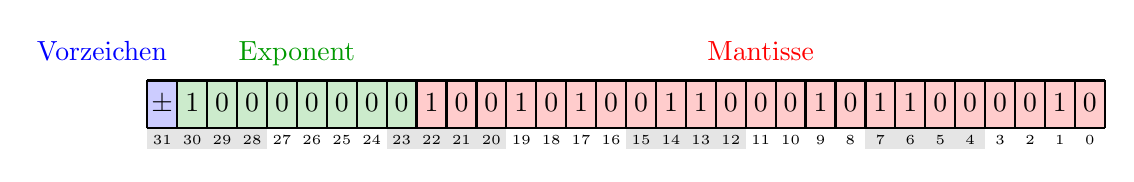
\begin{tikzpicture}[>=latex,thick,scale=0.38]

\definecolor{darkgreen}{rgb}{0,0.6,0}
\fill[color=blue!20]      (0,-0.8) rectangle (1,0.8);
\fill[color=darkgreen!20] (1,-0.8) rectangle (9,0.8);
\fill[color=red!20]       (9,-0.8) rectangle (32,0.8);

\node[color=blue]      at ( 1  ,0.8) [above left] {Vorzeichen\strut};
\node[color=darkgreen] at ( 5  ,0.8) [above] {Exponent\strut};
\node[color=red]       at (20.5,0.8) [above] {Mantisse\strut};

\fill[color=gray!20] ( 0,-0.8) rectangle ( 4,-1.5);
\fill[color=gray!20] ( 8,-0.8) rectangle (12,-1.5);
\fill[color=gray!20] (16,-0.8) rectangle (20,-1.5);
\fill[color=gray!20] (24,-0.8) rectangle (28,-1.5);

\foreach \k in {0,...,31}{
	\node at ({31.5-\k},{-1.2}) {\tiny \k};
}

\draw (0,0.8)--(32,0.8);
\foreach \x in {0,...,32}{
	\draw (\x,-0.8)--(\x,+0.8);
}
\draw (0,-0.8)--(32,-0.8);

\def\feld#1#2{
\node at ({#1+0.5},0) {$\mathstrut #2$};
}

\feld{0}{\pm}

\feld{1}{1}
\feld{2}{0}
\feld{3}{0}
\feld{4}{0}
\feld{5}{0}
\feld{6}{0}
\feld{7}{0}
\feld{8}{0}

\feld{9}{1}
\feld{10}{0}
\feld{11}{0}
\feld{12}{1}
\feld{13}{0}
\feld{14}{1}
\feld{15}{0}
\feld{16}{0}
\feld{17}{1}
\feld{18}{1}
\feld{19}{0}
\feld{20}{0}
\feld{21}{0}
\feld{22}{1}
\feld{23}{0}
\feld{24}{1}
\feld{25}{1}
\feld{26}{0}
\feld{27}{0}
\feld{28}{0}
\feld{29}{0}
\feld{30}{1}
\feld{31}{0}

\end{tikzpicture}
\end{center}
Die Ganzzahl $\texttt{10000000}_2=128_{10}$ im Exponentenfeld
muss um $127$ verringert werden um den Exponenten $1$ zu ergeben.

Die grösste und kleinste mit einem \texttt{float} darstellbare Zahl ist
somit
\begin{align*}
\texttt{1.11111111111111111111111}_2 \cdot 2^{\phantom{-}128}
&=
3.4028232_{10}\cdot 10^{\phantom{-}38}
\\
\texttt{1.00000000000000000000000}_2 \cdot 2^{-127}
&=
5.8774717_{10}\cdot 10^{-39}
\end{align*}
Den 24 binären Mantissenbits entsprechen gut 7 Dezimalstellen.

\begin{table}
\centering
\renewcommand\arraystretch{1.15}
\begin{tabular}{|l|>{$}l<{$}|>{$}l<{$}|>{$}l<{$}|}
\hline
&\texttt{float}&\texttt{double}&\texttt{long double}\\
\hline
kleinste darstellbare Zahl    &
	1.17549\cdot 10^{-38}&2.22507\cdot 10^{-308}&3.3621\cdot 10^{-4932}\\
grösste darstellbare Zahl     &
	3.40282\cdot10^{38} &1.79769\cdot10^{308} &1.18973\cdot10^{4932}\\
$\varepsilon$                 &
	1.19209\cdot 10^{-7}&2.22045\cdot 10^{-16}&1.0842\cdot 10^{-19}\\
kleinster Exponent            & -125&-1021&-16381\\
grösster Exponent             & 128&1024&16384\\
kleinste denormalisiert Zahl: &
	1.4013\cdot 10^{-45}&4.94066\cdot 10^{-324}&3.6452\cdot 10^{-4951}\\
\hline
\end{tabular}
\caption{Eigenschaften der Gleitkommatypen \texttt{float}, \texttt{double}
und \texttt{long double}.
Die Zeile $\varepsilon$ ist die Differenz zwischen 1 und der kleinsten
darstellbaren Zahl, die grösser ist als $1$.
Einzelne Exponentenwerte haben eine spezielle Bedeutung (siehe Text),
daher fallen die kleinstmöglichen Exponenten grösser aus als aufgrund
ihrer Bitlänge zu erwarten ist.
\label{buch:table:limits}}
\end{table}


\begin{table}
\centering
\begin{tabular}{|l|c|c|c|c|}
\hline
Typ&Bytes&Mantisse&Exponent&IEEE-754\\
\hline
\texttt{half},
\texttt{binary16}    &\phantom{0}2& \phantom{0}10 & \phantom{0}5     & * \\
\texttt{float},
\texttt{binary32}    &\phantom{0}4& \phantom{0}23 & \phantom{0}8     & * \\
\texttt{extended} 
                     &\phantom{0}5& \phantom{0}29 & 10               &   \\
\texttt{double},
\texttt{binary64}    &\phantom{0}8& \phantom{0}52 & 11               & * \\
\texttt{double extended},
\texttt{long double} &          10& \phantom{0}63 & 15               & * \\
\texttt{quad}
\texttt{binary128}   &          16& 112           & 15               & * \\
\texttt{binary256}   &          32& 236           & 19               & * \\
\hline
\end{tabular}
\caption{Übliche Gleitkommatypen mit Länge der Mantisse und des Exponenten.
Die meisten Compiler implementieren nur \texttt{float} und \texttt{double},
manchmal auch noch \texttt{long double}.
Die im Standard IEEE 754-2008 definierten Typen sind in der letzten Spalte
mit einen $*$ versehen.
\label{buch:table:ieee754}}
\end{table}

\subsubsection{Gebräuchliche Formate}
Der 1985 verabschiedete Standard IEEE~754 beschreibt die heute gebräuchlichen
Implementation von Gleitkommatypen abschliessend.
Damit ist gewährleistet, dass numerische Rechnungen auf verschiedenen
Prozessoren reproduzierbare Resultate geben.

Die C++-Standardbibliothek bietet im \texttt{<limits>} Header die Möglichkeit, 
Informationen über die Datentypen zu erhalten.
In Tabelle~\ref{buch:table:limits} sind die Resultate für die
gebräuchlichsten Typen zusammengestellt.
Allerdings offenbart sich hier auch ein Problem dieser Implementation
von \texttt{<limits>}.
Wie wir weiter unten sehen werden, definiert der IEEE 754 Standard
Werte für $\pm\infty$, die kleiner sind als die angegebenen
maximalen Werte.

Aktuelle Compiler unterstützen typischerweise die Gleitkomma-Typen
\texttt{float}, \texttt{double} und \texttt{long double}.
Bei Mikrokontrollern, wo Berechnungen mit der hohen Präzision
eines \texttt{double} nur schon wegen des Platzedarfs der Werte
und des Zeitbedarfs für die Operationen kaum sinnvoll sind, ist oft
nur der \texttt{float}-Typ implementiert.
Der GNU-Compiler für die 8-bit AVR-Prozessorfamilie stellt behandelt
zum Beispiel \texttt{double} genau gleich wie \texttt{float}.
Graphikkarten unterstützen oft noch einen halben Gleitkommatyp
\texttt{binary16}, dessen Genauigkeit für die Darstellung von 3D-Objekten
ausreichend ist.

\subsubsection{Rundung}
Der IEEE 754 Standard schreibt auch vor, wie Resultate gerundet werden
müssen.
\index{Rundungs-Regel}
Bei vielen Operationen entstehen Resultate, die einen längeren 
Nachkommateil haben als in das gegeben Gleitkommaformat passt,
das Resultat muss gerundet werden.
Der Standard kennt fünf verschiedene Rundungsverfahren und empfiehlt,
dass die Funktionen wie Wurzeln, Exponentialfunktionen,
trigonometrische Funktionen und viele weitere so implementiert werden 
müssen, dass das Resultat korrekt gerundet ist.
Damit ist gemeint, dass das Resultat entsteht, in dem auf das
mathematisch exakte Resultat die gewählt Rundungs-Regel angewendet
wird.

Der Standard bezweckt mit diesen, dass man sich im Rahmen der
Rundungsgenauigkeit auch auf die letzte Stelle eines Gleitkommawertes
verlassen kann.
Dies ist keinen Selbstverständlichkeit.
Gleitkomma-Implementationen von GPUs beispielsweise erfüllen diese
\index{GPU}
Bedingung oft nicht und garantieren in ihren Spezifikation manchmal
nur korrekte Resultate mit Ausnahme der letzten 1-2 bits.

\subsubsection{Die Null}
Die Gleitkomma-Darstellung definiert, dass die Mantisse ein implizites
führends \texttt{1}-bit hat. 
In diesem Format lässt sich die Null aber nicht darstellen, es ist
also eine separate Definition nötig:
\begin{itemize}
\item Vorzeichen $\texttt{0}$ oder $\texttt{1}$ erlaubt die Unterscheidung
zwischen $+0$ und $-0$.
\item Alle Exponentenbits $=\texttt{0}$.
\item Alle Mantissenbits $=\texttt{0}$.
\end{itemize}
Dies ist ein Spezialfall einer denormalisierten Zahl (siehe weiter unten)

\subsubsection{Unendlich grosse Werte}
Im Laufe einer numerischen Berechnung kann es vorkommen, dass die Resultate
so gross werden, dass nicht mehr im gegebenen Gleitkommatyp gespeichert
werden könne.
Der Standard verlangt, dass diese Situation durch einen spezielle Wert
für unendlich grosse Zahlen wiedergegeben werden kann, der wie
folgt definiert ist:
\begin{itemize}
\item Vorzeichenbit \texttt{0} oder \texttt{1} um zwischen
$+\infty$ und $-\infty$ unterscheiden zu können.
\item Alle Exponenten-Bits $= \texttt{1}$
\item Alle Mantissenbits $=\texttt{0}$
\end{itemize}
Dies bedeutet, dass der grösste nutzbare Exponent des $\texttt{float}$-Typs
nur noch $127$ ist.

\subsubsection{Denormalizierung}
\index{denormalisierte Zahl}%
Die Mantisse einer Gleitkommazahl beginnt immer mit einer 1, die aber
nicht gespeichert wird.
Wird eine Zahl kleiner als mit dem zur Verfügung stehenden Exponenten-Bereich
darstellbar, kann sie nicht mehr in diesem Format gespeichert werden.
Um solche Zahlen darzustellen, wurde vom Standard einem Exponenten aus
lauter \texttt{0} eine besondere Bedeutung gegeben.
Für den Typ \texttt{float} entspricht er nicht mehr dem Exponenten $-127$
sondern $-126$ und das implizite führend Bit der Mantisse ist jetzt 0.
Mit diesen sogenannten denormalisierten Zahlen lassen sich noch kleinere
Wert darstellen, die aber nicht mehr so präzis sind, weil sie weniger
signifikante Stellen aufweisen.

\subsubsection{Vor- und Nachteile}
\begin{itemize}
\item[$\oplus$] Konstanter relativer Fehler
\item[$\oplus$] Dank des grossen Wertebereiches sind Über- und Unterlauf
unwahrscheinlich.
\item[$\ominus$] Der kleinste Gleitkommatyp ist bereits so gross wie
der gebräuchlichste Ganzzahltyp,
Gleitkommazahlen brauchen mehr Platz.
\item[$\ominus$] Geschwindigkeit: sofern keine Hardware-Beschleunigung
zur Verfügung steht sind Gleitkomma-Operationen deutlich langsamer
als Operationen mit Festkomma-Zahlen.
\item[$\ominus$]
In einer Multi-Core CPU hat nicht unbedingt jeder Kern eine Gleitkomma-Einheit.
Gleitkommaoperationen in verschiedenen Threads können sich also gegenseitig
behindern.
\end{itemize}

\subsection{Hochpräzisionsbibliotheken
\label{buch:subsection:mp}}
TODO: GMP
